\subsubsection{Wersja podstawowa modelu ze zmienną liczbą wierzchołków}

Dokładność modelu uczonego na grafach treningowych z liczbą wierzchołków od czterech do siedmiu,
prezentuje się dość stabilnie po początkowej fazie wzrostu. Występują tylko drobne fluktuacje.
Po kilku początkowych epokach, dokładność oscyluje wokół 95\%, dochodząc nawet do 100\%.
Linie walidacji i treningu są bardzo blisko siebie, co sugeruje dobrą generalizację modelu
i nie wskazuje na przeuczenie.

W przypadku straty modelu, początkowy gwałtowny spadek sugeruje, że model dość szybko się uczy.
Po 10 epokach następuje stabilizacja straty na niskim, bo wynoszącym około 0.1, poziomie.
Podobnie jak w przypadku dokładności, strata dla zbioru walidacyjnego jest blisko straty treningowej.
Można zaobserować pewne wzrosty, które mogą być spowodowane trudniejszymi przypadkami w zbiorze walidacyjnym.

\begin{figure}[ht]
	\centering
	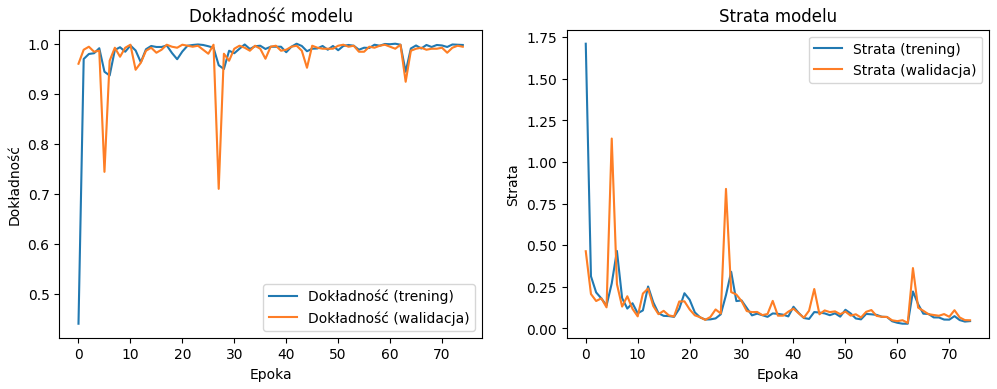
\includegraphics[height=5.5cm]{resources/tests/images/v3/multiple_edges_img.png}
	\caption{Dokładność i walidacja dla modelu ze zmienną liczbą wierzchołków}
	\label{Fig:tests-var-0a}
\end{figure}
\FloatBarrier

Model ten wydaje się być dobrze dopasywany i stabilny oraz poprawnie generalizujący.
Z uwagi na bliskość wyników dla treningu i walidacji, można stwierdzić, że model nie jest przeuczony.

\begin{figure}[ht]
	\centering
	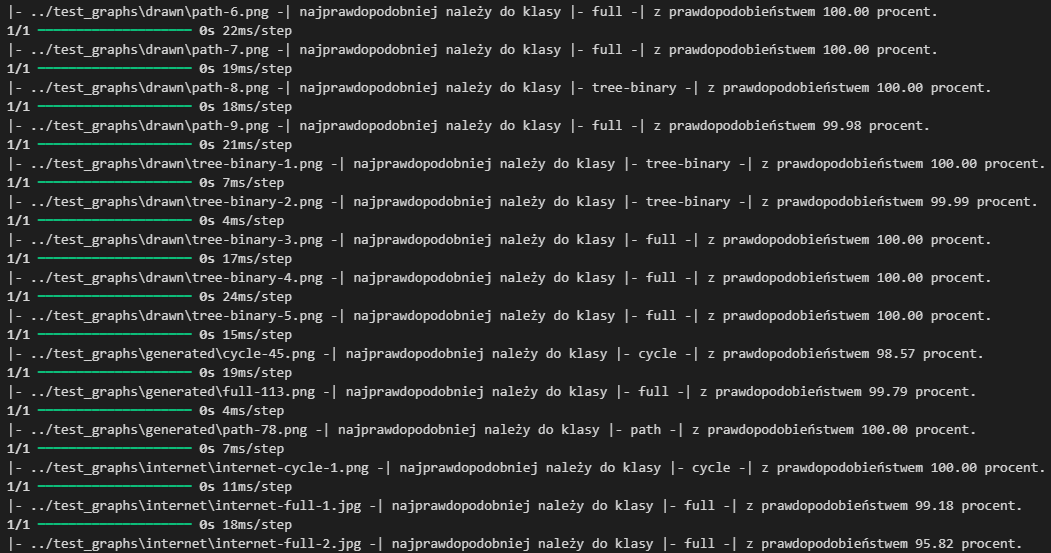
\includegraphics[width=14cm]{resources/tests/images/v3/multiple_edges_txt.png}
	\caption{Klasyfikacja obrazów zewnętrznych dla modelu ze zmienną liczbą wierzchołków}
	\label{Fig:tests-var-0b}
\end{figure}
\FloatBarrier

\begin{figure}[ht]
	\centering
	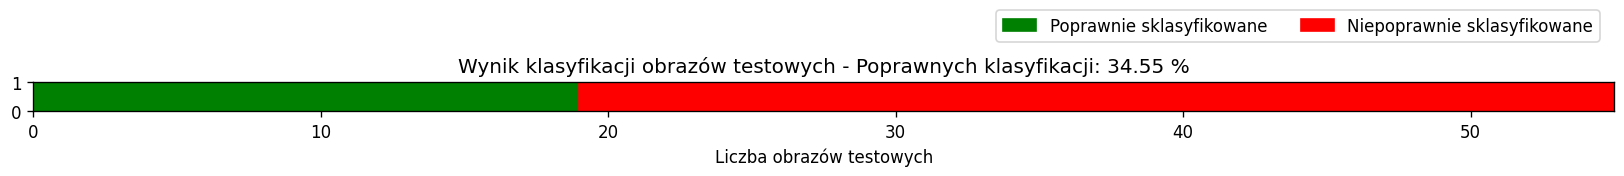
\includegraphics[width=14cm]{resources/tests/images/v3/multiple_edges_bar.png}
	\caption{Wizualizacja klasyfikacji obrazów zewnętrznych dla modelu ze zmienną liczbą wierzchołków}
	\label{Fig:tests-var-0c}
\end{figure}
\FloatBarrier

Model poprawnie sklasyfikował ponad 34\% rysunków zewnętrznych.
Nie jest to zły wynik, biorąc pod uwagę niską złożoność modelu.

\begin{figure}[ht]
	\centering
	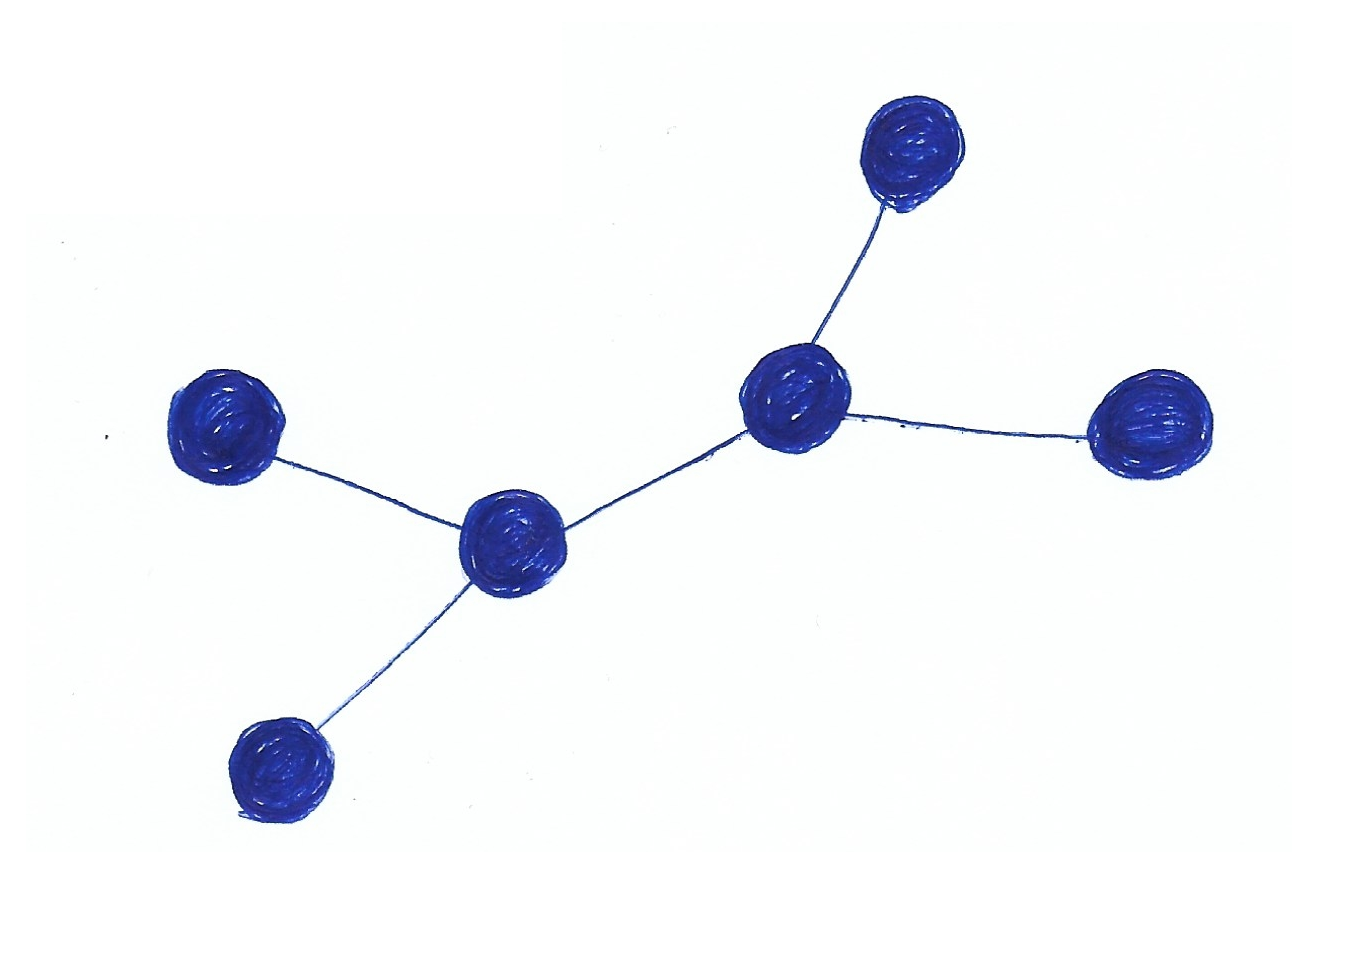
\includegraphics[width=10cm]{../graph_classification/test_graphs/drawn/tree-binary-1.png}
	\caption{Klasyfikacja przykładowego grafu zewnętrznego przez model ze zmienną liczbą wierzchołków.
		Przypisana klasa to drzewo binarne z 100\% pewnością.}
	\label{Fig:tests-var-0d}
\end{figure}
\FloatBarrier

\subsubsection{Zmodyfikowany model ze zmienną liczbą wierzchołków - Conv2D i Droput oraz spowolnienie uczenia}

W modelu wprowadzone zostało zwiększenie liczby filtrów dla warstw Conv2D, zwiększenie parametru Dropout
oraz zastosowano wywołanie zwrotne, które spowalnia uczenie.

Dokładność treningowa i walidacyjna modelu bardzo szybko wzrasta do wartości bliskich 100\%
i stabilizuje się na takim poziomie do końca procesu nauki.
Gdyby tylko dokładność treningowa osiągała taki poziom, możnaby założyć z dużą dozą pewności, przeuczenie modelu.
W tym przypadku jednak, różnice między dokładnością walidacyjną a treningową są marginalne.

Straty modelu wykazują podobne cechy do dokładności - szybki spadek wartości oraz stabilizacja na niskim poziomie.

\begin{figure}[ht]
	\centering
	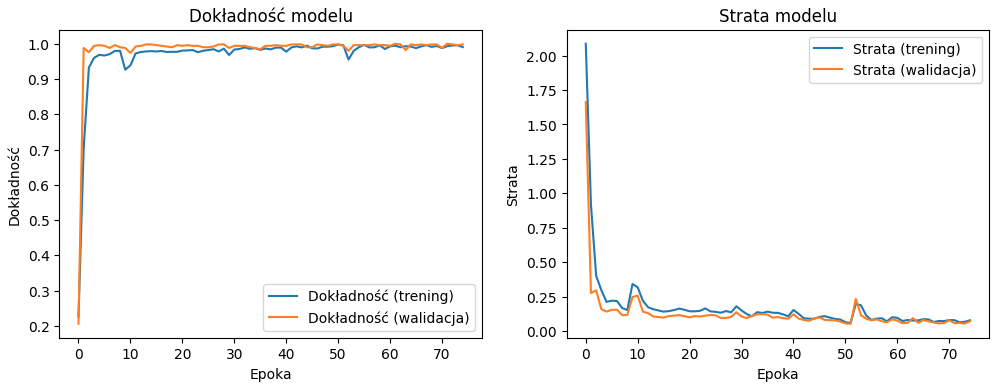
\includegraphics[width=14cm]{resources/tests/images/v4/multiple_edges_1_img.png}
	\caption{Dokładność i walidacja dla zmodyfikowanego modelu ze zmienną liczbą wierzchołków - Conv2D i Droput}
	\label{Fig:tests-var-1a}
\end{figure}
\FloatBarrier

Wydaje się, że model osiągnął pewną stabilność na niskim poziomie, co może pozytywnie świadczyć o jego zdolności generalizacji na nowe dane.

\begin{figure}[ht]
	\centering
	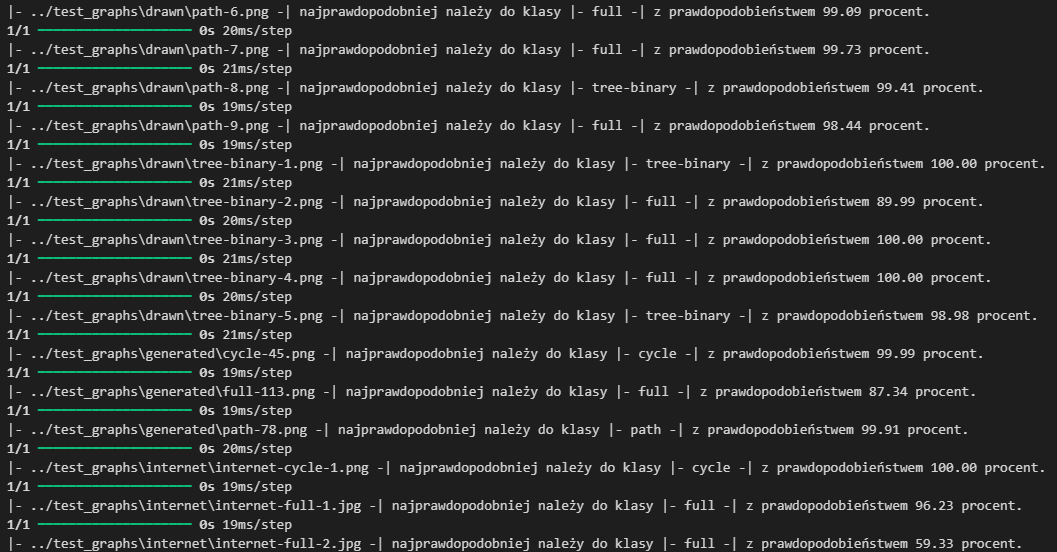
\includegraphics[width=14cm]{resources/tests/images/v4/multiple_edges_1_txt.png}
	\caption{Klasyfikacja obrazów zewnętrznych dla zmodyfikowanego modelu ze zmienną liczbą wierzchołków - Conv2D i Droput}
	\label{Fig:tests-var-1b}
\end{figure}
\FloatBarrier

\begin{figure}[ht]
	\centering
	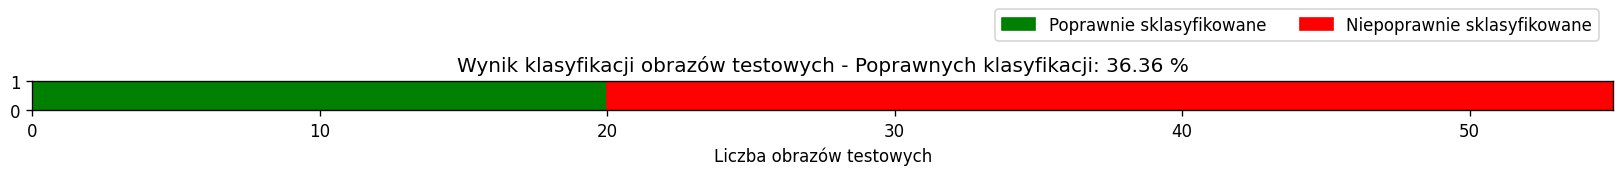
\includegraphics[width=14cm]{resources/tests/images/v4/multiple_edges_1_bar.png}
	\caption{Wizualizacja klasyfikacji obrazów zewnętrznych dla zmodyfikowanego modelu ze zmienną liczbą wierzchołków - Conv2D i Droput}
	\label{Fig:tests-var-1c}
\end{figure}
\FloatBarrier

Osiągnięta stabilizacja modelu i brak znaczących różnic między wartościami dokładności,
czy straty na zbiorach treningowych i wdalidacyjnych, nie przełożyła się w sposób rewolucyjny na osiągi modelu.
Model jednakże nie wypadł całkowicie źle - poprawnie sklasyfikował 36\% zewnętrznych grafów testowych,
co plasuje go w czołówce testowanych modeli pod kątem realnej dokładności.

\begin{figure}[ht]
	\centering
	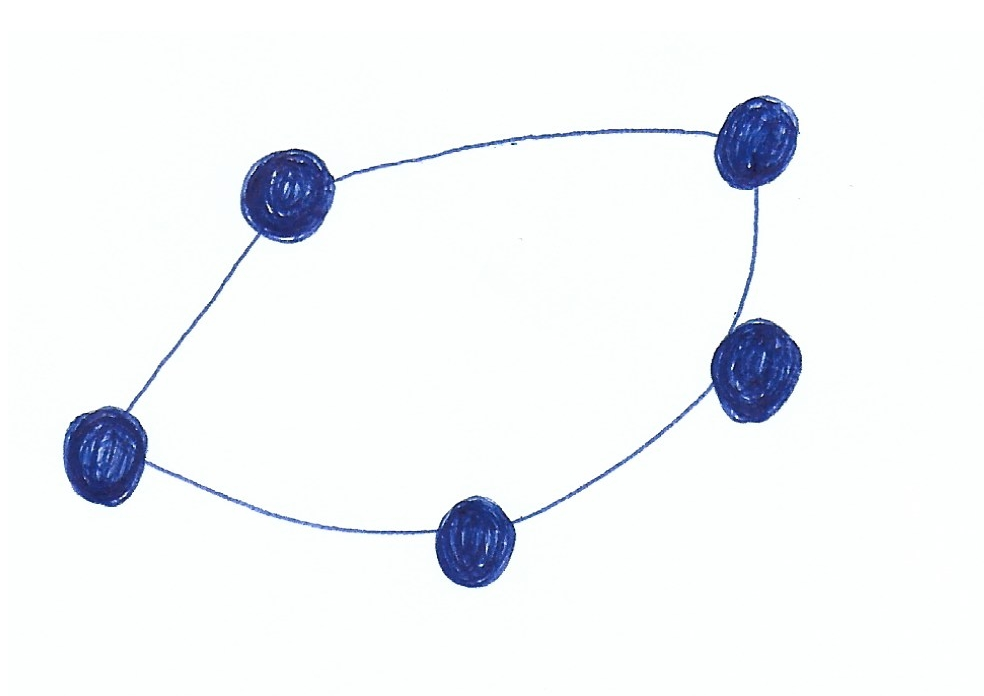
\includegraphics[width=10cm]{../graph_classification/test_graphs/drawn/cycle-7.png}
	\caption{Klasyfikacja przykładowego grafu zewnętrznego przez zmodyfikowany model ze zmienną liczbą wierzchołków
		- Conv2D i Droput oraz spowolnienie uczenia.
		Przypisana klasa to cykl z 98,88\% pewnością.}
	\label{Fig:tests-var-1d}
\end{figure}
\FloatBarrier

\subsubsection{Zmodyfikowany model ze zmienną liczbą wierzchołków - modyfikacje połączone}

Do modelu wprowadzone zostały modyfikacje na wzór tych ze zmodyfikowanego modelu z walidacją krzyżową.
Przetestowany został wariant z włączonymi wszystkimi modyfikacjami na raz.

Podobnie jak dla zmodyfikowanego modelu z walidacją krzyżową, dokładność treningowa jest bardzo wysoka (prawie 100\%),
ale dokładność walidacyjna nie jest ustabilizowana. Jej wartości oscylują w przedziale od 0,2, aż do 0,9.
To sugeruje, że model nie generalizuje dobrze na nowych danych i może być nadmiernie dopasowany.

Wykresy straty prezentują się w podobny sposób jak i wykresy dokładności.
Strata treningowa jest bliska zeru, co mówi o świetnym zapamiętywaniu danych treningowych przez model, kosztem generalizacji na nowe dane.
Strata walidacji jednak jest niestabilna z bardzo wysokimi wartościami w niekórych epokach.

\begin{figure}[ht]
	\centering
	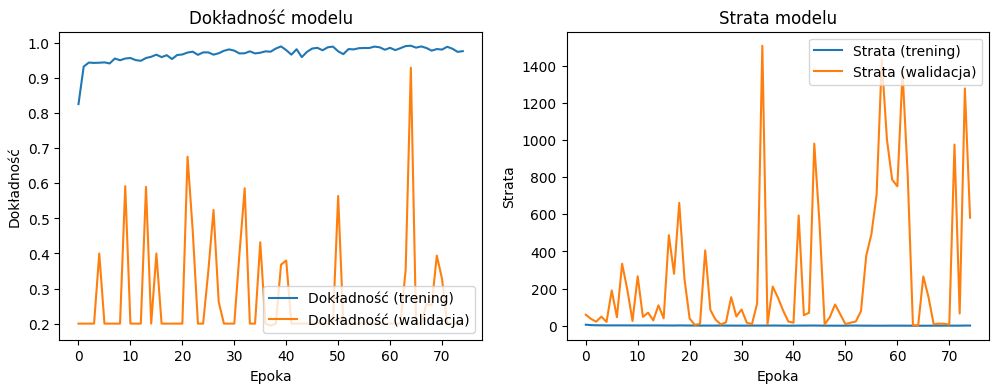
\includegraphics[width=14cm]{resources/tests/images/v4/multiple_edges_img.png}
	\caption{Dokładność i walidacja dla w pełni zmodyfikowanego modelu ze zmienną liczbą wierzchołków}
	\label{Fig:tests-var-2a}
\end{figure}
\FloatBarrier

Model wykazuje cechy modelu przeuczonego.
Są to bardzo wysoka dokładność i niemal zerowa strata na zbiorze treningowym
oraz bardzo niska dokładność i wysoka, ale niestabilna strata na zbiorze walidacyjnym.
Wniosek jaki można wyciągnąć jest taki, że model zapamiętał dane treningowe, ale nie nauczył się żadnych wzorców.

\begin{figure}[ht]
	\centering
	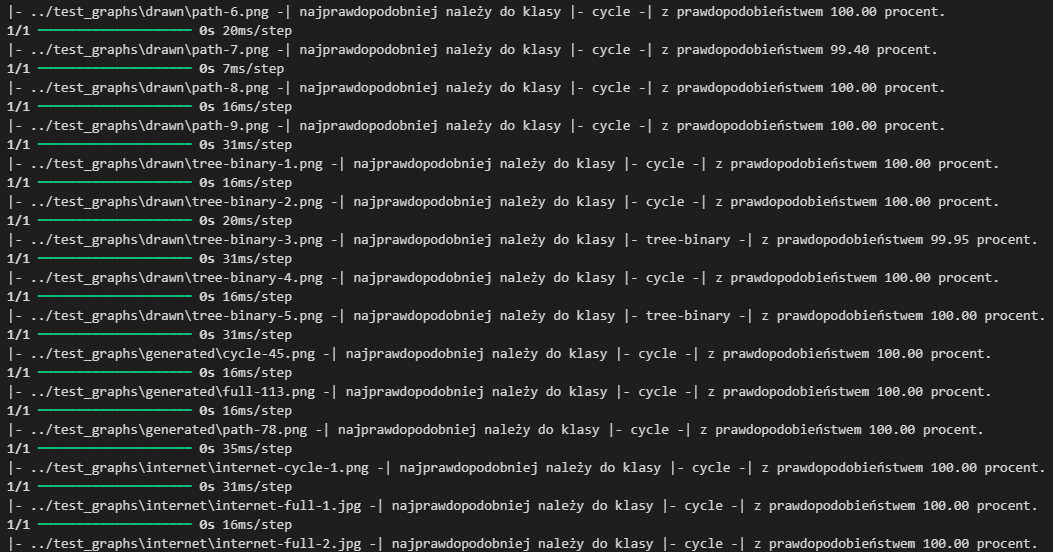
\includegraphics[width=14cm]{resources/tests/images/v4/multiple_edges_txt.png}
	\caption{Klasyfikacja obrazów zewnętrznych dla w pelni zmodyfikowanego modelu ze zmienną liczbą wierzchołków}
	\label{Fig:tests-var-2b}
\end{figure}
\FloatBarrier

\begin{figure}[ht]
	\centering
	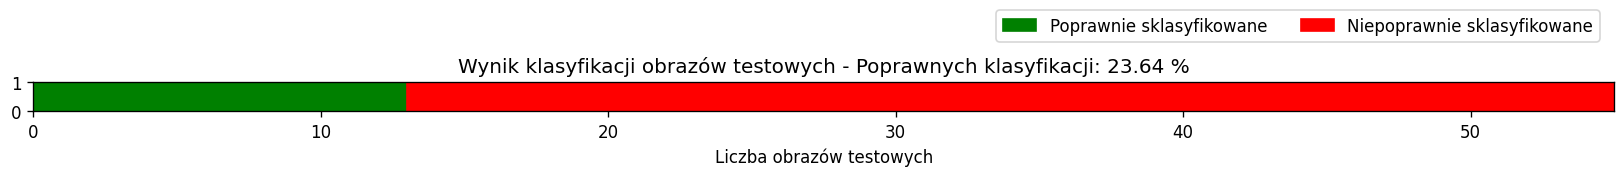
\includegraphics[width=14cm]{resources/tests/images/v4/multiple_edges_bar.png}
	\caption{Wizualizacja klasyfikacji obrazów zewnętrznych dla w pelni zmodyfikowanego modelu ze zmienną liczbą wierzchołków}
	\label{Fig:tests-var-2c}
\end{figure}
\FloatBarrier

Model poprawnie wskazał tylko około 24\% grafów, lecz analiza jego wskaźników mówi nam,
że jest to dzieło raczej przypadku, aniżeli poprawnego nauczenia się ogólnych wzorców danych.
Jego dokładność walidacyjna była bardzo niestabilna.

\begin{figure}[ht]
	\centering
	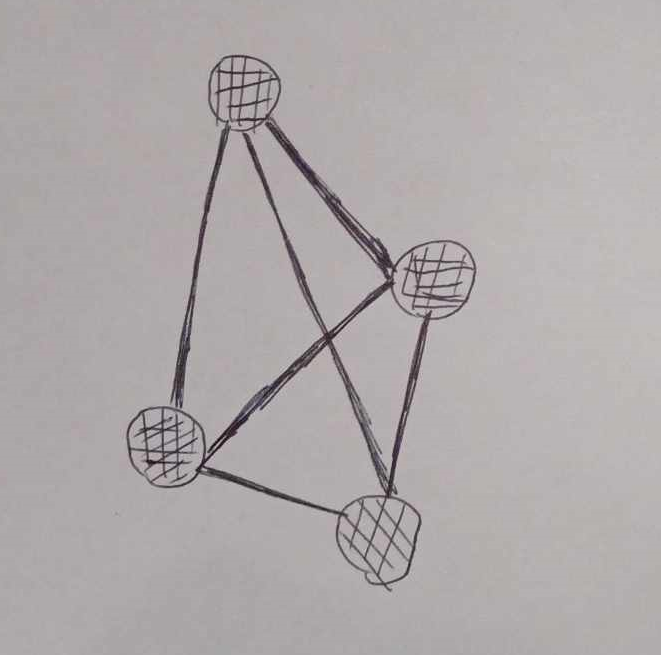
\includegraphics[width=10cm]{../graph_classification/test_graphs/drawn/full-3.png}
	\caption{Klasyfikacja przykładowego grafu zewnętrznego przez zmodyfikowany model ze zmienną liczbą wierzchołków - modyfikacje połączone
		Przypisana klasa to ścieżka z 99,68\% pewnością.}
	\label{Fig:tests-cv-2d}
\end{figure}
\FloatBarrier